\section{Exploring the incidents' classification}

\subsection*{Question 4.1}
\textit{Incidents have two types: the type of the incident at the moment it was reported (Initial Type Group) and the type of the incident after it has been studied and classified (Event Clearance Group). Obviously, there should be some kind of correlation of the latter with the former (for instance, incidents reported as robberies are very likely to be also classified finally as robberies). How strong is this correlation?}

The visualization uses a heatmap to show this correlation.
The rows show the incident types at the moment it was reported, while the columns show the type it was classified as (we will refer to it as the ``final'' type).
Each cell in the map contains a square, whose area and color are proportional to the number of record for the particular row and column.
Color uses a continuos heat colormap.

The order of rows and columns is initially alphabetical.
However, this order does not have any particular meaning, since there is no $1$-to-$1$ mapping between the categorical values of \textit{Initial Type Group} and \textit{Event Clearance Group}.
Starting from such an order, we have manually moved some rows and columns to types which seems to be possibly correlated, in order to show this correlation along the main diagonal.
For example, \textit{Initial Type Group} has the value \textit{Parking Violation}, but \textit{Event Clearance Group} does not have it:
we have it closed to \textit{Traffic Related Calls}.

\cref{fig:4_1_initial_vs_final_group_heatmap} shows the visualization.
We can see that:
\begin{itemize}
    \item After some reordering of columns, most of the big squares are along the main diagonal. This means there is a high correlation between the initial and final types of incidents.
    \item In many cases there is a match between the initial and final type (e.g. \textit{Disturbances}). Nevertheless, in some cases a single initial type matches multiple more specific final types (e.g. \textit{Theft} matches \textit{Car prowl}, \textit{Other property} and \textit{Shoplifting}).
    \item The first row of the table has a different behaviour and represents the incidents without an initial type. This group matches different final types, mostly \textit{Disturbances}, \textit{Suspicious circumstances} and \textit{Traffic related calls}.
\end{itemize}

\begin{figure}[h]
	\centering
	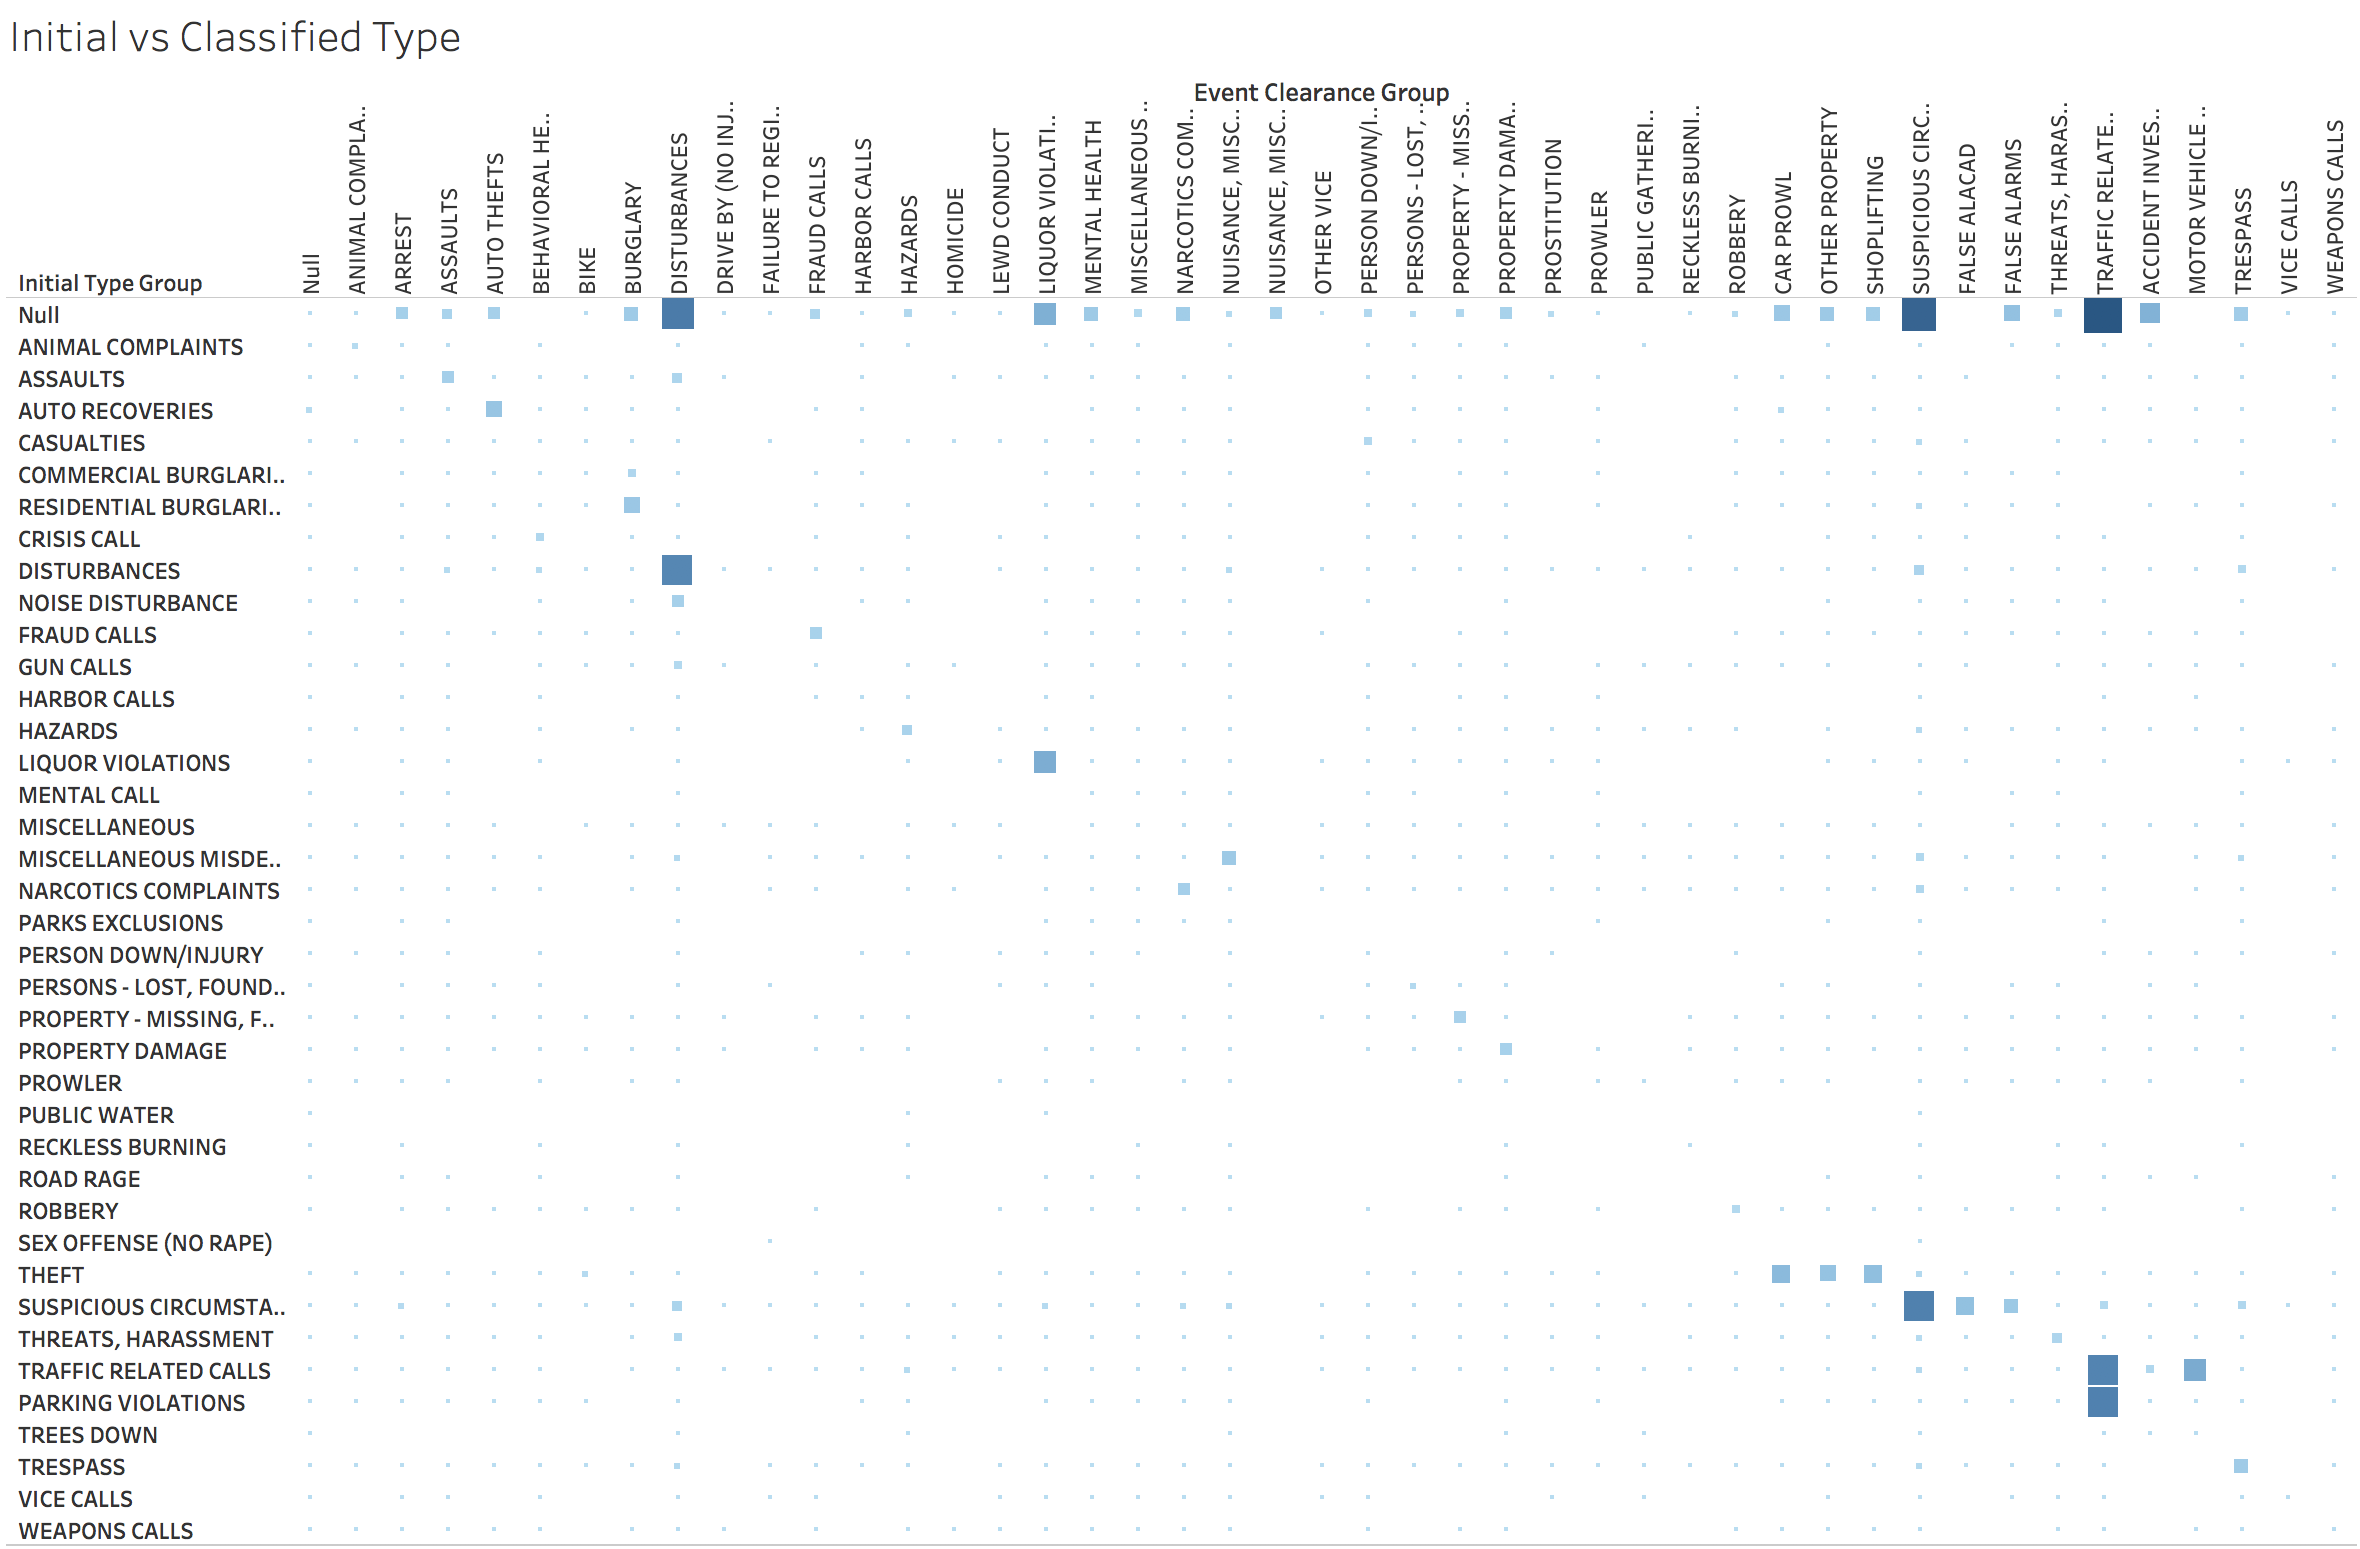
\includegraphics[width=\columnwidth]{figures/4_1_initial_vs_final_group_heatmap}
	\caption{Correlation between the initial and final incident type. The sheet is called \textit{Initial vs Final Type} in Tableau.}
	\label{fig:4_1_initial_vs_final_group_heatmap}
\end{figure}

The visualization answers the question, but requires some manual work to find the matching between initial and final types.
Moreover, it wastes a lot of space, since most initial types are highly correlated to only a few final ones.
This makes the square dedicated to interesting correlations very small and difficult to compare with the others.
The use of colors as an overloading helps with that, by does not really solve the problem. 

To better visualize the interesting correlations and remove the manual reordering step, we use a treemap.
We filter out values without an initial type since we have discussed this case previously.
We use the initial type for the first split for the treemap.
Each rectangle corresponds to a pair initial and final types.
Both the color and the area of each rectangle encode the number of elements for the particular pair.
Tooltips allow the user to interactively get additional information for each rectangle, namely initial type, final type and number of matching incidents.

\cref{fig:4_1_initial_vs_final_group_treemap} shows the visualization:
\begin{itemize}
	\item There are some very big rectangles, which indicates a high correlation between the initial and final types.
	\item There are many small rectangles, which indicates a low correlation. For most types the area occupied from small rectangles is negligible, but for some other (e.g. \textit{Suspicious circumstances}) this area is quite relevant. This fact was very difficult to spot in the previous visualization.
	\item Mapping between the initial and final types do not need to be specified interactively by the user. This is the biggest improvement over the previous design.
\end{itemize}

To sum up, there is a quite strong correlation between initial and final types.
However, a lot of incidents with some particular initial cases are often classified in a different way afterwards (e.g. \textit{Suspicious circumstances}).

\begin{figure}[h]
	\centering
	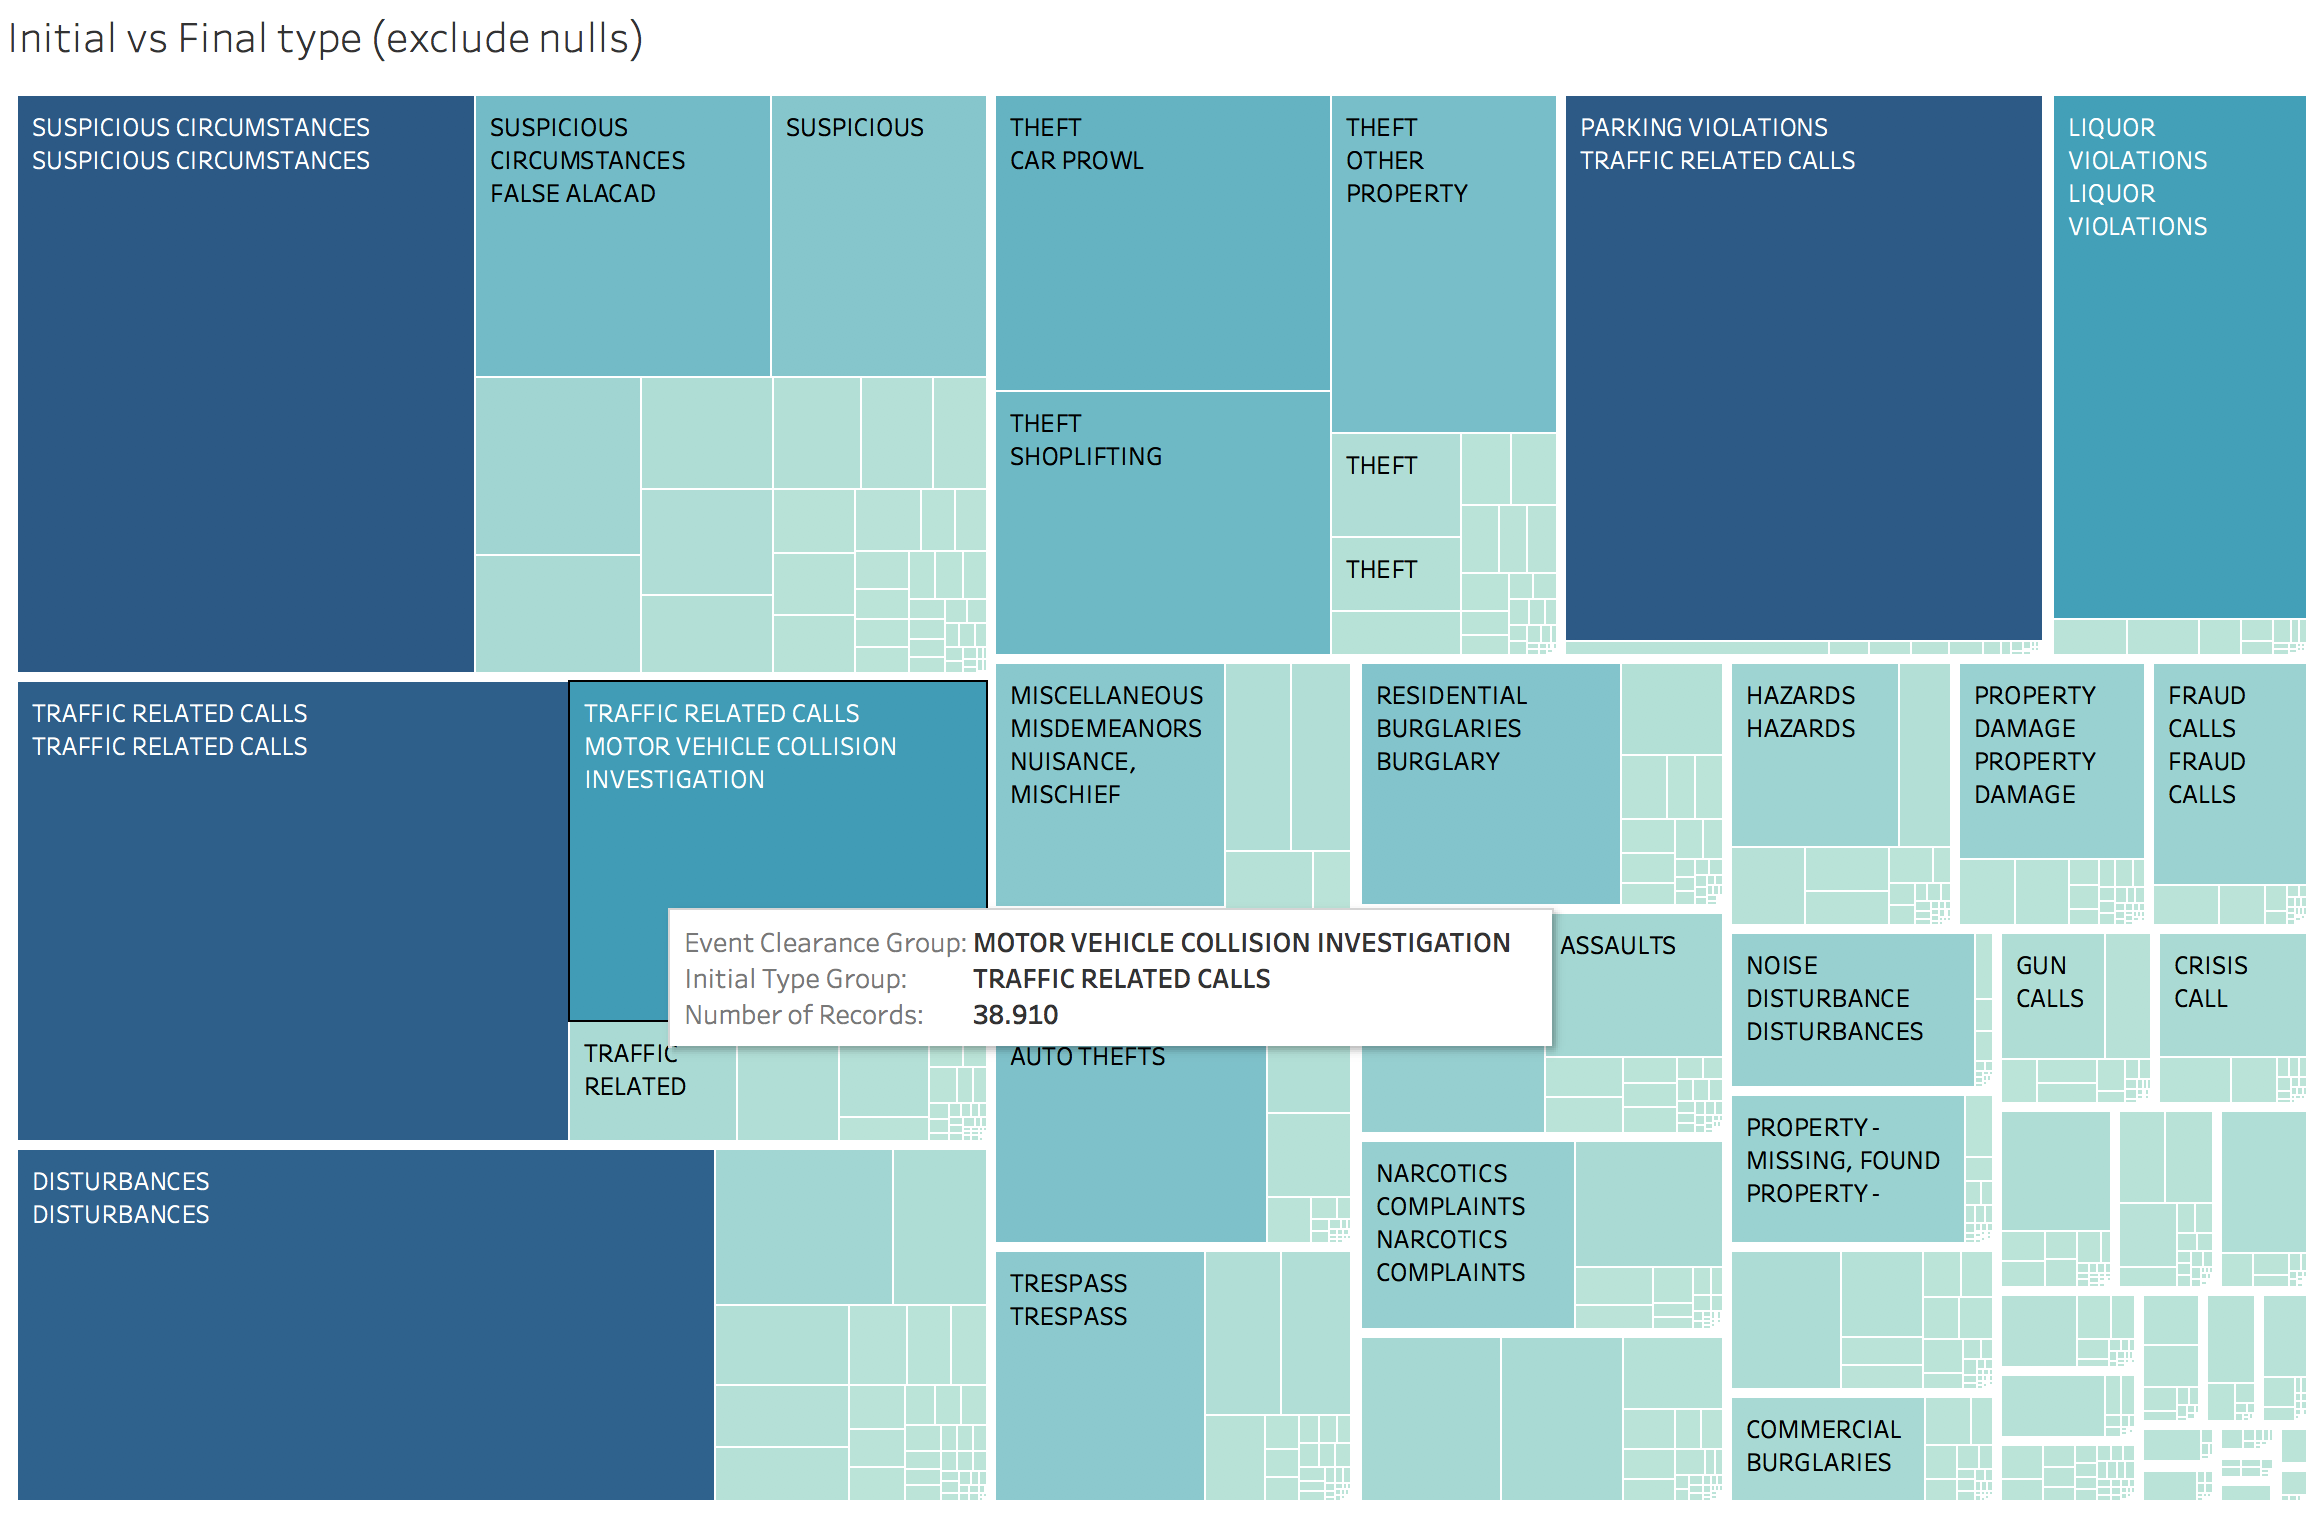
\includegraphics[width=\columnwidth]{figures/4_1_initial_vs_final_group_treemap}
	\caption{Correlation between the initial and final incident type (excluding incidents without an initial type). The sheet is called \textit{Initial vs Final Type (exclude nulls)} in Tableau.}
	\label{fig:4_1_initial_vs_final_group_treemap}
\end{figure}


\subsection*{Question 4.2}
\textit{How do the total number of incidents break down per incident reported type (Initial Type Group) and incident resolution type (Event Clearance Group)?}

To answer this question we have created $2$ treemaps very similar to \cref{fig:4_1_initial_vs_final_group_treemap}.
The former is a shows first the initial and then the final types (including null values), the latter shows first the final and then the initial types.

% TODO: put screenshot of dashboard \textit{Incident Types Break-Down}.
% To complete the dashboard, we add $2$ histogram to show the initial and final groups marginal distributions.

We can notice the following:
\begin{itemize}
	\item About $3/8$ of the incidents have no information about the initial type. Most of them are than classified in the most frequent final types (\textit{Traffic Related Calls}, \textit{Suspicious Circumstances}, \textit{Disturbances} etc.).
	\item There are $5$ main initial types of incidents that include about another $3/8$ of the total, namely \textit{Suspicious Circumstances}, \textit{Traffic Related Calls}, \textit{Disturbances}, \textit{Theft} and \textit{Parking Violations}.
	\item The remaining $2/8$ of the incidents are spread among different initial types.
	\item There is no the problem of missing data for the final type: less than $1\%$ of the incidents miss it.
	\item There are $4$ main final types of incidents that include about $1/2$ of the entries, namely \textit{Traffic Related Calls}, \textit{Suspicious Circumstances}, \textit{Disturbances} and \textit{Liquor Violations}.
	\item The remaining $1/2$ is distributed among the other types.
	\item In most cases, the majority of incidents in each final type group matches the initial type. There is thus a correlation between the initial and final incident type, as said for Question 4.1
\end{itemize}


\subsection*{Question 4.3}
\textit{How do the total number of incidents break down per incident resolution type (Event Clearance Group) and incident resolution subtype (Event Clearance Subgroup)?}

The visualization uses a treemap, since groups and subgroups can naturally be organized in a tree hierarchy.
Each group is represented by a rectangle, which can be divided in sub-rectangles to represent the subgroups, if any.
Both color and area of the rectangles encode the number of incidents with the given type / subtype.

\begin{figure}[h]
	\centering
	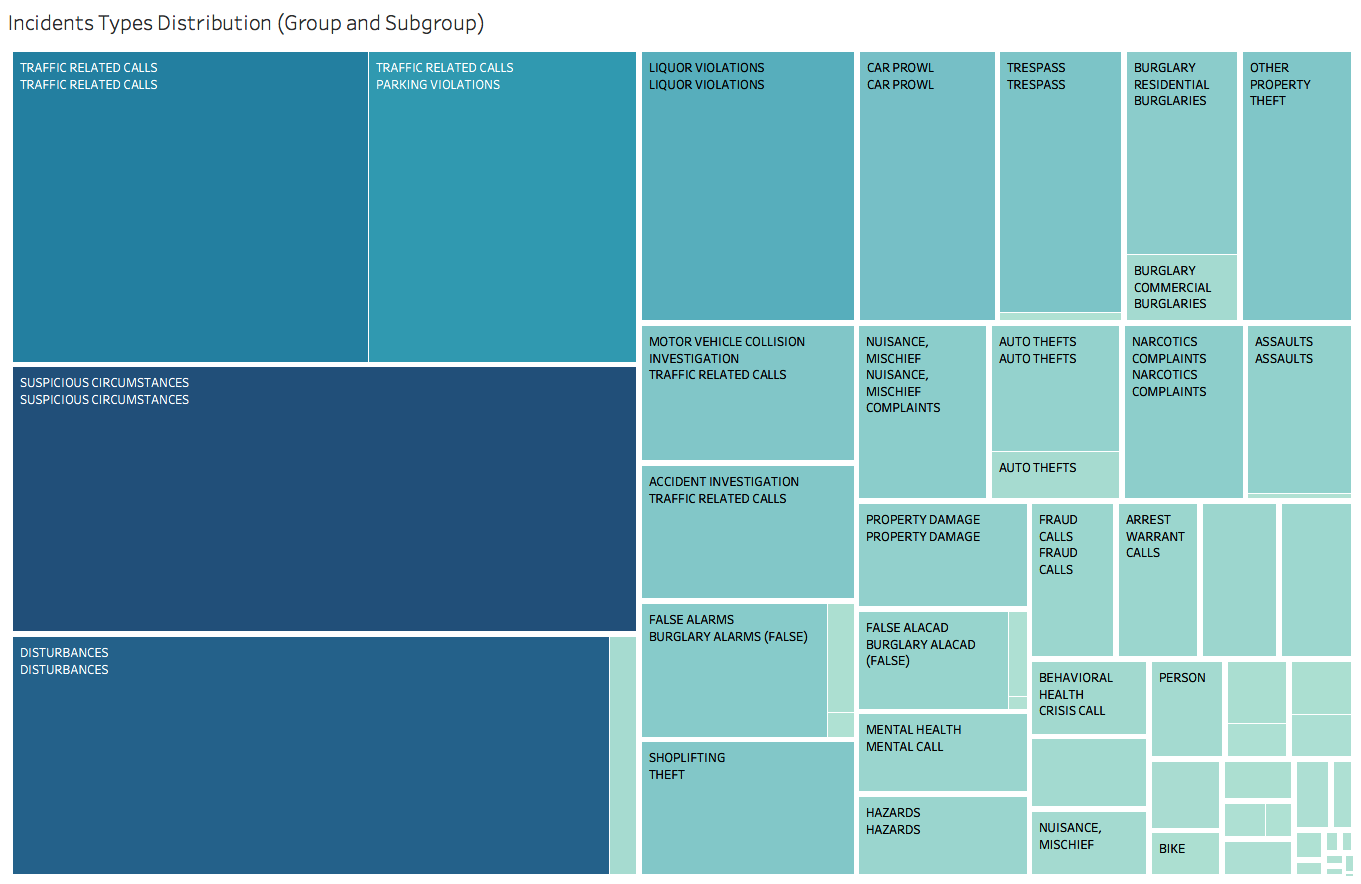
\includegraphics[width=\columnwidth]{figures/4_3_groups_subgroups}
	\caption{Incidents by Type and Subtype. The sheet is called \textit{Incidents Types Distribution (Group and Subgroup)} in Tableau.}
	\label{fig:4_3_groups_subgroups}
\end{figure}

\cref{fig:4_3_groups_subgroups} shows the visualization.
We can see that:
\begin{itemize}
	\item There are $4$ types that include about $50\%$ of all of incidents, namely \textit{Traffic Related Calls}, \textit{Suspicious Circumstances}, \textit{Disturbances} and \textit{Liquor Violations}.
	\item Only $10$ out of $45$ type groups have subtypes.
	\item Groups that are divided in subgroups have only $2$ or $3$ of them.
	\item In most cases there is a dominant subgroups that includes most of the cases; the only exception is the group \textit{Traffic Related Calls}, where incidents are distributed almost equally in both subgroups \textit{Traffic Related Calls} and \textit{Parking Violations}.
\end{itemize}
